\chapter{Analiză și Fundamentare Teoretică}
\label{ch:analysis}
\pagestyle{fancy}

\section{Cerințe funcționale și non-funcționale}
%%%%%%%%%%%%%%%%%%%%%%%%%%%%%%%%%%%%%%%%%%%%%%%%%%%%%%%%%%%%%%%%%%%%%%%%%%%%%%%%%%%%%%%%%%%%%%%%%%%%%%%%%%%%%%%%%%%%%%%%%%%%%%%%%%%%%%%%%%%%%%%%%%%%%%%%%%
\subsection{Cerințe funcționale}
\begin{itemize}
    \setlength\itemsep{0.5em}
    \item Pentru un utilizator neautentificat, sunt realizabile următoarele acțiuni:
    \begin{itemize}
		\setlength\itemsep{0.5em}
        \item Accesare pagină de Logare
        \item Accesare pagină de Creare cont nou
        \item Încercare de logare
        \item Încercare de creare cont nou
    \end{itemize}
    \item Pentru un utilizator autentificat, sunt realizabile următoarele acțiuni:
    \begin{itemize}
		\setlength\itemsep{0.5em}
        \item Accesare pagină de Dashboard
        \begin{itemize}
            \setlength\itemsep{0.5em}
            \item Adăugare text în caseta de text
            \item Trimitere text spre procesare prin apăsarea butonului de Submit
            \item Vizualizare rezultate
            \item Generare grafic pentru vizualizarea evoluției cuvintelor cheie extrase într-o perioadă de timp selectată de utilizator
            \item Salvare articol (text analizat și rezultatele obținute)
        \end{itemize}
        \item Accesare pagină de Profil
        \begin{itemize}
            \setlength\itemsep{0.5em}
            \item Editare câmp nume
            \item Editare câmp prenume
            \item Editare câmp nume de utilizator, cu condiția să nu fie atribuit altui cont
            \item Editare câmp email, cu condiția să nu fie atribuit altui cont
            \item Editare câmp parolă
        \end{itemize}
        \item Accesare pagina de Trenduri
        \begin{itemize}
            \setlength\itemsep{0.5em}
            \item Generare grafic pentru vizualizarea celor mai populare 10 subiecte într-o perioadă de timp selectată de utilizator
            \item Vizualizarea unui WordCloud, constituit din cuvintele cheie sau expresiile extrase din textele analizate
        \end{itemize}
        \item Accesare pagină de Evoluție
        \begin{itemize}
            \setlength\itemsep{0.5em}
            \item Generare grafic pentru vizualizarea numărului de apariții pentru un cuvânt ales și o perioadă de timp selectată de utilizator
        \end{itemize}
        \item Accesare pagină de Istoric
        \begin{itemize}
            \setlength\itemsep{0.5em}
            \item Vizualizare articole salvate în istoric
            \item Accesarea analizei detaliate a unui articol selectat
            \item Ștergerea unui articol selectat
        \end{itemize}
    \end{itemize}
\end{itemize}
\newpage

\subsection{Cerințe pentru funcții de analiză a unui text}
\begin{itemize}
    \setlength\itemsep{0.5em}
    \item Funcție de analiză a sentimentelor dintr-un text financiar
    \item Funcție de sumarizare a unui text
    \item Funcție de extragere a cuvintelor
\end{itemize}
%%%%%%%%%%%%%%%%%%%%%%%%%%%%%%%%%%%%%%%%%%%%%%%%%%%%%%%%%%%%%%%%%%%%%%%%%%%%%%%%%%%%%%%%%%%%%%%%%%%%%%%%%%%%%%%%%%%%%%%%%%%%%%%%%%%%%%%%%%%%%%%%%%%%%%%%%%
\subsection{Cerințe non-funcționale}
\begin{itemize}
    \setlength\itemsep{0.5em}
    \item Securitatea
    \begin{itemize}
        \setlength\itemsep{0.5em}
        \item Pentru a accesa anumite resurse, utilizatorul trebuie mai întâi să își creeze un cont, apoi să se logheze în aplicație
        \item La crearea contului, înainte să fie salvată, parola trece print-o funcție de hashing cu salt, cu scopul de a avea un rezultat diferit pentru același input al mai multor utilizatori, daca va fi cazul
        \item La logarea în aplicație se generează un token pentru a putea autoriza utilizatorul atunci când dorește să acceseze anumite resurse
    \end{itemize}
    \item Compatibilitatea
    \begin{itemize}
        \setlength\itemsep{0.5em}
        \item Aplicația a fost creată și rulată utilizând ca sistem de operare Windows OS
        \item Pentru a utiliza alt sistem de operare, spre exemplu MacOS, singura diferență este baza de date, fiind necesar găsirea unui echivalent al Microsoft SQL Server Management
    \end{itemize}
\end{itemize}

%%%%%%%%%%%%%%%%%%%%%%%%%%%%%%%%%%%%%%%%%%%%%%%%%%%%%%%%%%%%%%%%%%%%%%%%%%%%%%%%%%%%%%%%%%%%%%%%%%%%%%%%%%%%%%%%%%%%%%%%%%%%%%%%%%%%%%%%%%%%%%%%%%%%%%%%%%

\section{Cazuri de utilizare}
Folosind îndrumările din~\cite{UseCasesGuidlines} pentru crearea și detalierea cazurilor de utilizare a aplicației, trebuie avute în vedere următoarele aspecte: 
\begin{enumerate}
    \setlength\itemsep{0.5em}
    \item {\it Enunțarea precondițiilor}, adică a stării sau stărilor în care sistemul se află înaintea începerii executării operațiunilor specifice cazului de utilizare
    \item {\it Descrierea flow-ului principal}, care trebuie să acopere următoarele: când și unde începe cazul, când cazul de utilizare interacționează cu actorii și când schimbă date, când cazul folosețe date stocate sau dorește să stocheze datele, când și cum este finalizat cazul
    \item {\it Descrierea flow-ului alternativ}, care trebuie să descrie ce se întâmplă cu sistemul în cazurile în care apare o eroare
    \item {\it Enunțarea postcondițiilor}, adică a stării sau stărilor în care sistemul ajunge după ce cazul este finalizat
  \end{enumerate}
%%%%%%%%%%%%%%%%%%%%%%%%%%%%%%%%%%%%%%%%%%%%%%%%%%%%%%%%%%%%%%%%%%%%%%%%%%%%%%%%%%%%%%%%%%%%%%%%%%%%%%%%%%%%%%%%%%%%%%%%%%%%%%%%%%%%%%%%%%%%%%%%%%%%%%%%%%
\subsection{Utilizator neautentificat}

\begin{figure}[h]
	\centering
	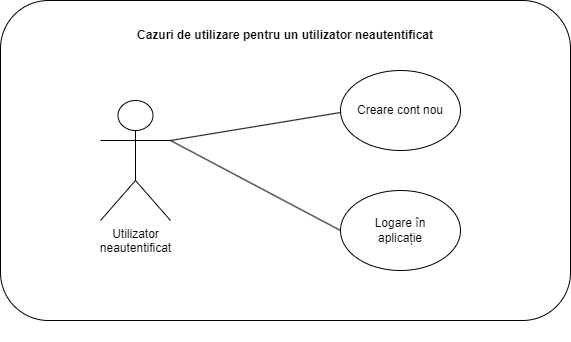
\includegraphics[width=100mm]{figs/useCaseUnauthenticated.png}
    \caption{Cazuri de utilizare pentru un utilizator neautentificat}
	\label{fig:useCaseUnauthenticated}
\end{figure}

\subsubsection{Descrierea cazurilor de utilizare pentru un utilizator neautentificat în figura \ref{fig:useCaseUnauthenticated}}
\begin{enumerate}
    \item Creare cont nou 
    \begin{itemize}
        \setlength\itemsep{0.5em}
        \item Un utilizator neautentificat poate să acceseze pagina de creare cont nou și să se înregistreze în aplicație
        \item Precondiții: utilizatorul neautentificat trebuie să se afle pe pagina de Creare cont nou
        \item Flow principal
        \begin{enumerate}
            \item Utilizatorul neautentificat introduce informațiile necesare: nume, prenume, nume de utilizator, email și parola
            \item Utilizatorul apasă pe butonul de trimitere
            \item Crearea unui nou cont a fost realizată cu succes și utilizatorul este redirecționat la pagina de logare în aplicație
        \end{enumerate}
        \item Flow alternativ
        \begin{enumerate}
            \item Utilizatorul neautentificat introduce informațiile necesare: nume, prenume, nume de utilizator, email și parola
            \item Utilizatorul apasă pe butonul de trimitere
            \item Emailul sau numele de utilizator deja sunt folosite de alt cont
            \item Flow-ul este reluat
        \end{enumerate}
        \item Postcondiții: Dacă a fost creat cu succes contul, utilizatorul este redirecționat la pagina de logare în aplicație
    \end{itemize}

    \item Logare
    \begin{itemize}
        \setlength\itemsep{0.5em}
        \item Un utilizator neautentificat poate să acceseze pagina de logare și să intre în aplicație, dacă acesta are deja un cont creat
        \item Precondiții: utilizatorul neautentificat trebuie să se afle pe pagina de logare
        \item Flow principal
        \begin{enumerate}
            \item Utilizatorul neautentificat introduce informațiile necesare: nume de utilizator sau email și parola
            \item Utilizatorul apasă pe butonul de trimitere
            \item Logarea s-a făcut cu succes și utilizatorul este acum autentificat și redirecționat la pagina de Dashboard
        \end{enumerate}
        \item Flow alternativ
        \begin{enumerate}
            \item Utilizatorul neautentificat introduce informațiile necesare: nume de utilizator sau email și parola
            \item Utilizatorul apasă pe butonul de trimitere
            \item Credențialele sunt greșite
            \item Flow-ul este reluat
        \end{enumerate}
        \item Postcondiții: Dacă utilizatorul s-a logat în aplicație, este redirecționat la pagina de Dashboard
    \end{itemize}
  \end{enumerate}

%%%%%%%%%%%%%%%%%%%%%%%%%%%%%%%%%%%%%%%%%%%%%%%%%%%%%%%%%%%%%%%%%%%%%%%%%%%%%%%%%%%%%%%%%%%%%%%%%%%%%%%%%%%%%%%%%%%%%%%%%%%%%%%%%%%%%%%%%%%%%%%%%%%%%%%%%%
\newpage
\subsection{Utilizator autentificat}
\begin{figure}[ht]
	\centering
	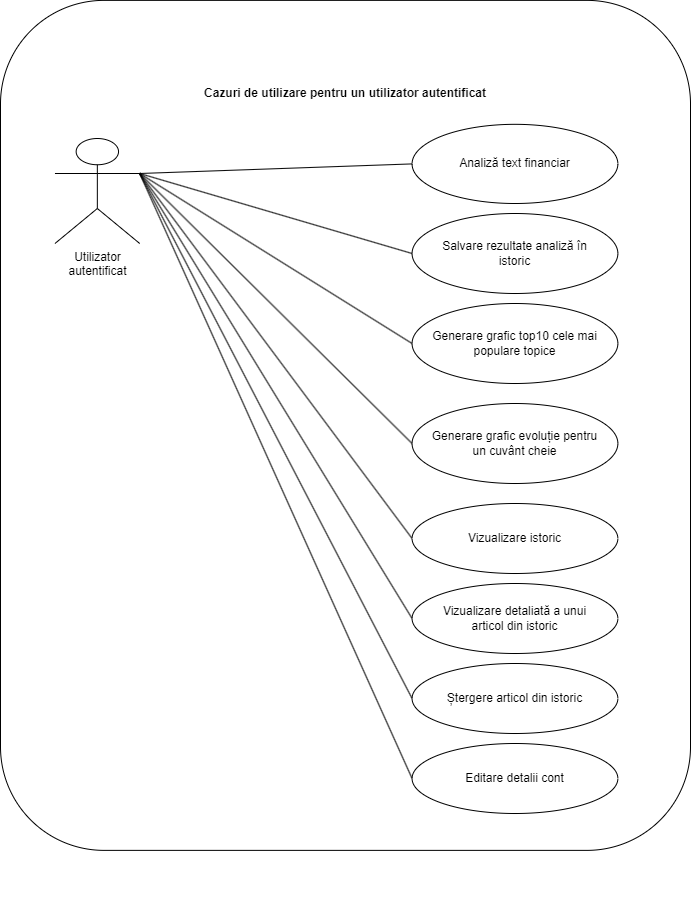
\includegraphics[width=100mm]{figs/useCasesAuthenticated.png}
    \caption{Cazuri de utilizare pentru un utilizator autentificat}
	\label{fig:useCasesAuthenticated}
\end{figure}
\subsubsection{Descrierea cazurilor de utilizare pentru un utilizator autentificat în figura \ref{fig:useCasesAuthenticated}}
\begin{enumerate}
    \setlength\itemsep{0.5em}
    \item Analizare text financiar
    \begin{itemize}
        \setlength\itemsep{0.5em}
        \item Un utilizator autentificat poate să introducă un text financiar și să îl obțină o analiză detaliată
        \item Precondiții: utilizatorul autentificat trebuie să se afle pe pagina de Dashboard
        \item Flow principal
        \begin{enumerate}
            \setlength\itemsep{0.5em}
            \item Utilizatorul autentificat introduce textul
            \item Utilizatorul apasă pe butonul de trimitere
            \item Apare un buton pentru a-l trimite pe utilizator într-o pagină cu rezultatele obținute în urma analizei
        \end{enumerate}
        \item Flow alternativ
        \begin{enumerate}
            \setlength\itemsep{0.5em}
            \item Utilizatorul autentificat introduce textul
            \item Utilizatorul apasă pe butonul de trimitere
            \item Modelul care trebuie să transmită rezultatele încă se încarcă
            \item Flow-ul este reluat
        \end{enumerate}
        \item Postcondiții: Dacă textul a fost analizat și apare butonul care îl trimite pe utilizator într-o pagină cu rezultatele obținute în urma analizei
    \end{itemize}

    \item Salvare rezultate analiză în istoric
    \begin{itemize}
        \setlength\itemsep{0.5em}
        \item Un utilizator autentificat poate să salveze rezultatele detaliate ale analizei textului
        \item Precondiții: utilizatorul autentificat trebuie să se afle în pagina de Dashboard, în partea cu toate informațiile detaliate
        \item Flow principal
        \begin{enumerate}
            \setlength\itemsep{0.5em}
            \item Utilizatorul autentificat apasă pe butonul de salvare
            \item Se deschide un modal pentru confirmare
            \item Se confirmă și articoul analizat este salvat în istoricul utilizatorului
        \end{enumerate}
        \item Postcondiții: Dacă utilizatorul a salvat articolul, acesta va apărea în tabelul din pagina de istoric
    \end{itemize}
\ \\
    Diagrama FlowChart se găsește în figura \ref{fig:saveArticleFlowchart}.
    \begin{figure}[H]
        \centering
        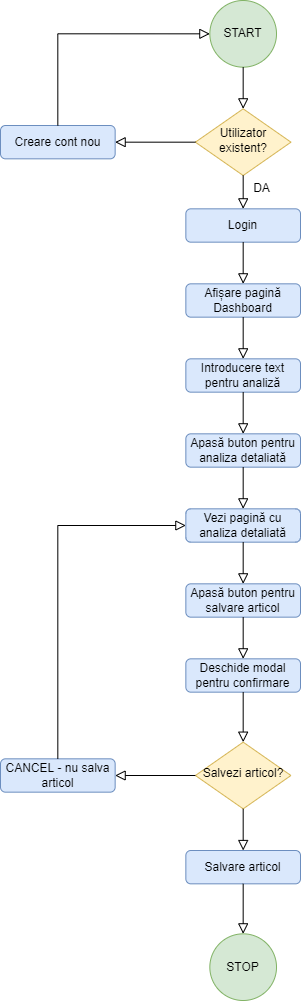
\includegraphics[height=100mm]{figs/saveArticleFlowchart.png}
        \caption{Diagramă FlowChart pentru salvarea rezultatelor unui text analizat în istoric}
        \label{fig:saveArticleFlowchart}
    \end{figure}

    \item Generare grafic pentru top 10 cele mai populare subiecte din aplicație
    \begin{itemize}
        \setlength\itemsep{0.5em}
        \item Un utilizator autentificat poate să genereze un grafic pentru a vedea top 10 cele mai populare cuvinte cheie (subiecte) din aplicație
        \item Precondiții: utilizatorul autentificat trebuie să se afle în pagina de Trending
        \item Flow principal
        \begin{enumerate}
            \setlength\itemsep{0.5em}
            \item Utilizatorul autentificat selectează o perioadă
            \item Utilizatorul apasă pe butonul de trimitere
            \item Apar rezultatele pe grafic
        \end{enumerate}
        \item Flow alternativ
        \begin{enumerate}
            \setlength\itemsep{0.5em}
            \item Utilizatorul autentificat selectează o perioadă
            \item Utilizatorul apasă pe butonul de trimitere
            \item Utilizatorul este notificat că nu există date din perioada selectată de acesta
            \item Flow-ul este reluat, selectând altă perioadă
        \end{enumerate}
        \item Postcondiții: Utilizatorul rămâne în pagina de Trending, având posibilitatea selectării altei perioade
    \end{itemize}

    \ \\
    Diagrama FlowChart se găsește în figura \ref{fig:trends}.
    \begin{figure}[H]
        \centering
        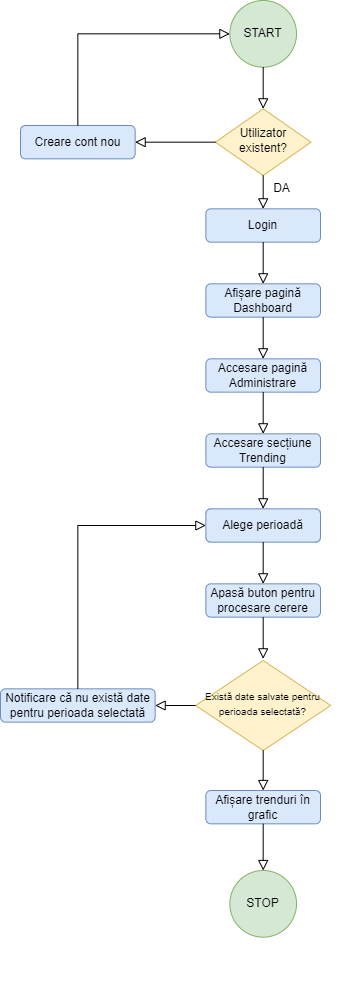
\includegraphics[height=100mm]{figs/trends.png}
        \caption{Diagramă FlowChart pentru generare grafic cu top 10 trenduri în aplicație}
        \label{fig:trends}
    \end{figure}

    \item Generare grafic pentru a vizualiza evoluția unui cuvânt cheie, într-o anumită perioadă
    \begin{itemize}
        \setlength\itemsep{0.5em}
        \item Un utilizator autentificat poate să genereze un grafic pentru a vedea evoluția unui cuvânt cheie, într-o anumită perioadă
        \item Precondiții: utilizatorul autentificat trebuie să se afle în pagina de Evoluție
        \item Flow principal
        \begin{enumerate}
            \setlength\itemsep{0.5em}
            \item Utilizatorul autentificat selectează o perioadă
            \item Utilizatorul autentificat introduce cuvântul
            \item Utilizatorul apasă pe butonul de trimitere
            \item Apar rezultatele pe grafic
        \end{enumerate}
        \item Flow alternativ
        \begin{enumerate}
            \setlength\itemsep{0.5em}
            \item Utilizatorul autentificat selectează o perioadă
            \item Utilizatorul autentificat introduce cuvântul
            \item Utilizatorul apasă pe butonul de trimitere
            \item Utilizatorul este notificat că nu există date, posibil din cauza perioadei sau din cauză că până acum nu a mai fost căutat cuvântul
            \item Flow-ul este reluat, selectând altă perioadă
        \end{enumerate}
        \item Postcondiții: Utilizatorul rămâne în pagina de Evoluție, având posibilitatea selectării altei perioade sau introducerii altui cuvânt
    \end{itemize}

    \item Vizualizare istoric
    \begin{itemize}
        \setlength\itemsep{0.5em}
        \item Un utilizator autentificat poate să vizualizeze istoricul
        \item Precondiții: utilizatorul autentificat poate să se afle în orice pagină
        \item Flow principal
        \begin{enumerate}
            \setlength\itemsep{0.5em}
            \item Utilizatorul autentificat selectează din bara de nagivare butonul de Istoric
            \item Utilizatorul este redirecționat la pagina de Istoric, unde poate vedea tabelul cu articolele salvate până acum
        \end{enumerate}
        \item Postcondiții: Utilizatorul este redirecționat la pagina de Istoric, unde poate vedea tabelul cu articolele salvate până acum
    \end{itemize}

    \item Vizualizarea detaliată a unui articol din istoric
    \begin{itemize}
        \setlength\itemsep{0.5em}
        \item Un utilizator autentificat poate să vizualizeze mai multe detalii ale unui articol salvat în istoric
        \item Precondiții: utilizatorul autentificat trebuie să se afle în pagina de Istoric
        \item Flow principal
        \begin{enumerate}
            \setlength\itemsep{0.5em}
            \item Utilizatorul autentificat apasă pe butonul de Vezi mai mult din dreptul articolului pe care dorește să îl redeschidă
            \item Apare un modal de confirmare
            \item Utilizatorul confirmă că vrea să revadă analiza acelui articol
            \item Utilizatorul este redirecționat în pagina de Dashboard, de această dată fără opțiunea de a salva articolul (pentru că acesta deja există în istoric)
        \end{enumerate}
        \item Flow alternativ
        \begin{enumerate}
            \setlength\itemsep{0.5em}
            \item Utilizatorul autentificat apasă pe butonul de Vezi mai mult din dreptul articolului pe care dorește să îl redeschidă
            \item Apare un modal de confirmare
            \item Utilizatorul nu confirmă că vrea să revadă analiza acelui articol
            \item Utilizatorul rămâne în pagina de Istoric
        \end{enumerate}
        \item Postcondiții: Utilizatorul este direcționat în pagina cu analiza detaliată a articolului selectat
    \end{itemize}


    \item Ștergere a unui articol din istoric
    \begin{itemize}
        \setlength\itemsep{0.5em}
        \item Un utilizator autentificat poate să șteargă un articol salvat în istoric
        \item Precondiții: utilizatorul autentificat trebuie să se afle în pagina de Istoric
        \item Flow principal
        \begin{enumerate}
            \setlength\itemsep{0.5em}
            \item Utilizatorul autentificat apasă pe butonul de Șterge din dreptul articolului pe care dorește să îl redeschidă
            \item Apare un modal de confirmare
            \item Utilizatorul confirmă că vrea să șteargă articolul
            \item Articolul este șters și tabelul este actualizat
        \end{enumerate}
        \item Flow alternativ
        \begin{enumerate}
            \setlength\itemsep{0.5em}
            \item Utilizatorul autentificat apasă pe butonul de Șterge din dreptul articolului pe care dorește să îl redeschidă
            \item Apare un modal de confirmare
            \item Utilizatorul nu confirmă că vrea să șteargă articolul
            \item Utilizatorul rămâne în pagina de Istoric și tabelul nu este actualizat
        \end{enumerate}
        \item Postcondiții: Se actualizează tabelul din istoricul utilizatorului și rămâne în pagina de Istoric
    \end{itemize}

    \ \\
    Diagrama FlowChart se găsește în figura \ref{fig:deleteArticle}.
    \begin{figure}[H]
        \centering
        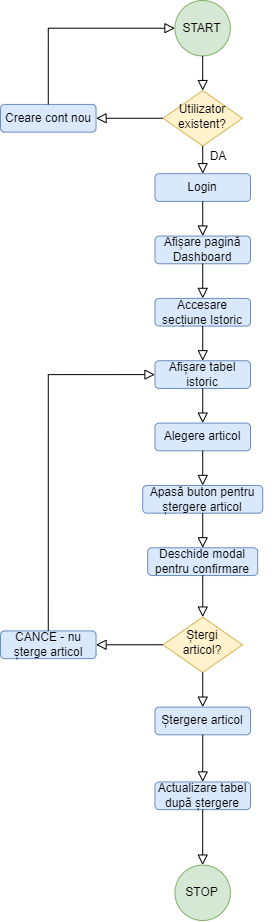
\includegraphics[height=110mm]{figs/deleteArticle.png}
        \caption{Diagramă FlowChart pentru ștergere articol din istoric}
        \label{fig:deleteArticle}
    \end{figure}

    \item Editare detalii cont
    \begin{itemize}
        \setlength\itemsep{0.5em}
        \item Un utilizator autentificat poate să editeze detaliile contului
        \item Precondiții: utilizatorul autentificat trebuie să se afle în pagina de Profil
        \item Flow principal
        \begin{enumerate}
            \setlength\itemsep{0.5em}
            \item Utilizatorul autentificat editează unul sau mai multe din câmpurile: nume, prenume, nume de utilizator, email, parolă nouă și confirmă parola
            \item Utilizatorul apasă pe butonul de trimitere
            \item Utilizatorul este notificat că detaliile contului au fost modificate cu succes
        \end{enumerate}
        \item Flow alternativ
        \begin{enumerate}
            \setlength\itemsep{0.5em}
            \item Utilizatorul autentificat editează unul sau mai multe din câmpurile: nume, prenume, nume de utilizator, email, parolă nouă și confirmă parola
            \item Unul dintre câmpurile de email sau nume de utilizator este deja folosit de alt cont
            \item Utilizatorul apasă pe butonul de trimitere
            \item Utilizatorul este notificat că email-ul sau numele de utilizator este deja folosit de alt cont
            \item Flow-ul este reluat
        \end{enumerate}
        \item Postcondiții: Detaliile contului au fost modificate cu succes
    \end{itemize}
  \end{enumerate}


%%%%%%%%%%%%%%%%%%%%%%%%%%%%%%%%%%%%%%%%%%%%%%%%%%%%%%%%%%%%%%%%%%%%%%%%%%%%%%%%%%%%%%%%%%%%%%%%%%%%%%%%%%%%%%%%%%%%%%%%%%%%%%%%%%%%%%%%%%%%%%%%%%%%%%%%%%
%%%%%%%%%%%%%%%%%%%%%%%%%%%%%%%%%%%%%%%%%%%%%%%%%%%%%%%%%%%%%%%%%%%%%%%%%%%%%%%%%%%%%%%%%%%%%%%%%%%%%%%%%%%%%%%%%%%%%%%%%%%%%%%%%%%%%%%%%%%%%%%%%%%%%%%%%%

\section{Algoritmi utilizați}
\subsection{Algoritmul pentru autorizarea accesului utilizatorului la anumite resurse}
Atunci când un utilizator nou își creează un cont și se loghează în aplicație, identitatea acestuia este verificată printr-un proces de autentificare. \\
Pentru a accesa anumite resurse, acesta trebuie să fie autorizat. Spre exemplu, pentru e efectua operații de ștergere a unor elemente importante, utilizatorul trebuie să aibă permisiunile necesare.
Așadar, pentru partea de autorizare utilizator, mecanismul este următorul: în momentul în care clientul trimite un request de logare în aplicație, se returnează un token pentru autorizarea requesturilor viitoare, dacă nu există deja unul. \\

Validarea tokenului pentru un anumit utilizator depinde de utilizator (pentru că serviciul folosește un map cu userId și token), de valabilitatea tokenului și dacă valoarea stocată în map corespunde cu valoarea transmisă pentru verificare. 
Dacă toate cele 3 condiții sunt îndeplinite, utilizatorul are permisiunea de a efectua operația pentru care s-a făcut această verificare.

\subsection{Algoritmul pentru crearea unei parole puternice}
O funcție de hashing este folosită pentru a lua un mesaj de o orice lungime, apoi în urma procesării, va rezulta un răspuns de lungime fixă.
Spre exemplu, funcția de hashing SHA512 va produce o valoarea de 512 biți, indiferent de lungimea valorii de intrare. Această funcție a fost folosită pentru a asigura securitatea parolei la înregistrarea unui utilizator nou.\\

Problema la funcțiile de hashing apare pentru că același input va produce același output de lungime fixă. 
Pentru a asigura unicitatea rezultatului, se folosește un {\it salt}, un set de caractere care sunt adăugate la finalul parolei, în acest caz, înainte să treacă prin funcția de hashing.


%%%%%%%%%%%%%%%%%%%%%%%%%%%%%%%%%%%%%%%%%%%%%%%%%%%%%%%%%%%%%%%%%%%%%%%%%%%%%%%%%%%%%%%%%%%%%%%%%%%%%%%%%%%%%%%%%%%%%%%%%%%%%%%%%%%%%%%%%%%%%%%%%%%%%%%%%%

\section{Protocoale utilizate}
\subsection{Protocolul HTTP}
Protocolul HTTP este un protocol utilizat pentru a transmite date între un server Web și un broswer (Google Chrome, Firefox, etc.). Se bazează pe protocolul de comunicare TCP/IP.\\
Se bazează pe mecanismul request-response, unde clientul (în acest caz, browserul) inițiază un request, apoi așteaptă un răspuns de la server.\\
Serverul procesează requestul primit de la client, apoi trimite răspunsul, după care conexiunea se întrerupe. Așadar, clientul și serverul sunt conectați doar pentru requestul și răspunsul curent, concluzionând astfel că 
protocolul HTTP este un protocol fără conexiune.\\
Tot din acest motiv, clientul și serverul nu rețin informații unul despre celalălalt, concluzionând că protocolul HTTP este un protocol fără stare, după cum putem afla din ~\cite{HTTPDefinition}.
\begin{figure}[H]
	\centering
	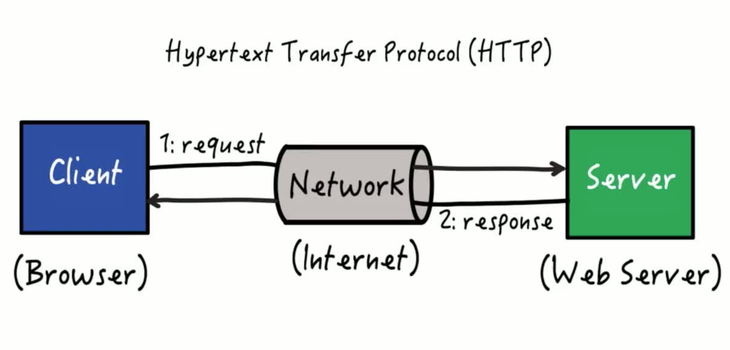
\includegraphics[width=100mm, scale=1]{figs/http.png}
    \caption{Protocolul HTTP. Sursa~\cite{HTTPDiagram}}
	\label{fig:http}
\end{figure}

\subsection{Protocolul TCP/IP}
Pentru SQL Server, protocolul TCP/IP se utilizează cel mai des, pentru că acesta permite dispozitivelor să comunice între diferite dispozitive.\\
De fiecare dată când se trimite ceva prin intermediul Internetului, modelul TCP/IP structurează informația în pachete pe care apoi le transmite prin cele 4 nivele: Aplicație, Transport, Internet, Acces rețea.
Informațiile sunt trimise în ordine, apoi sunt reasamblate în ordine inversă la celalalt capăt, așa cum este menționat aici~\cite{TCPDefinition}.\\

Protocolul TCP stabilește o conexiune între host-uri (server și baza de date, în acest caz), apoi asigură că pachetele de date sunt livrate.
\begin{figure}[H]
	\centering
	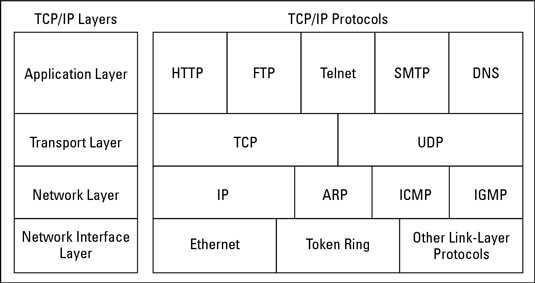
\includegraphics[width=100mm, scale=1]{figs/tcp.jpg}
    \caption{Modelul TCP/IP. Sursa~\cite{TCPDiagram}}
	\label{fig:tcp}
\end{figure}

%%%%%%%%%%%%%%%%%%%%%%%%%%%%%%%%%%%%%%%%%%%%%%%%%%%%%%%%%%%%%%%%%%%%%%%%%%%%%%%%%%%%%%%%%%%%%%%%%%%%%%%%%%%%%%%%%%%%%%%%%%%%%%%%%%%%%%%%%%%%%%%%%%%%%%%%%%
\subsection{Protocolul SMTP}
SMTP sau Simple Mail Transfer Protocol, este un protocol de email utilizat pentru a trimite mesaje dintr-un cont de email în altul, prin intermediul Internetului, bazat pe adresele de email.\\
Permite trimiterea unui mesaj spre unul sau mai mulți destinatari, includerea atașamentelor precum text, video, fotografii.\\
Atunci când un mail este trimis de la un client, acesta va ajunge la un server SMTP care e responsabil pentru transmiterea email-urilor mai departe, spre destinatar (serverul de mail al destinatarului).\\
De fiecare data când un mail este trimis, o conexiune se va deschide între serverul SMTP și serverul destinatar, care va asigura transmiterea datelor spre un destinatar valid. Altfel, email-ul revine la expeditor.
\begin{figure}[H]
	\centering
	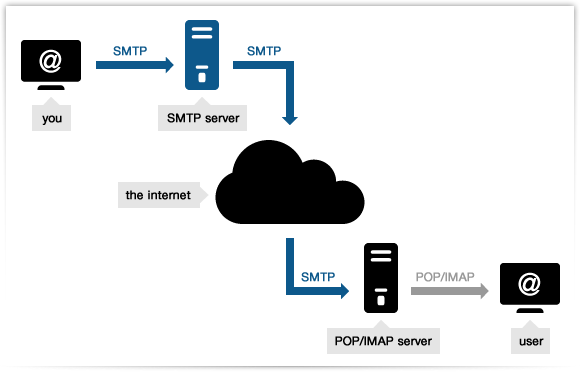
\includegraphics[width=100mm, scale=1]{figs/smtp.png}
    \caption{Protocolul SMTP. Sursa~\cite{SMTP}}
	\label{fig:smtp}
\end{figure}